\begin{frame}{Method}

\begin{itemize}
	\item Bigram-keystroke interval data: Dutch subset of copy-task corpus \parencite{waes2019,van2019multilingual}
	\item \textbf{Consonants task:} ``tjxgfl pgkfkq dtdrgt npwdvf''
	\item \textbf{LF-bigrams task:} ``een chaotische cowboy''
	\item Lexical and non-lexical copy-typing context
	\item Random sample of 250 ppts (18-25 years of age)
\end{itemize}

\end{frame}


% create the same graph without buffer decision
\begin{frame}{Copy-typing sequences of characters}
	
	\begin{center}
		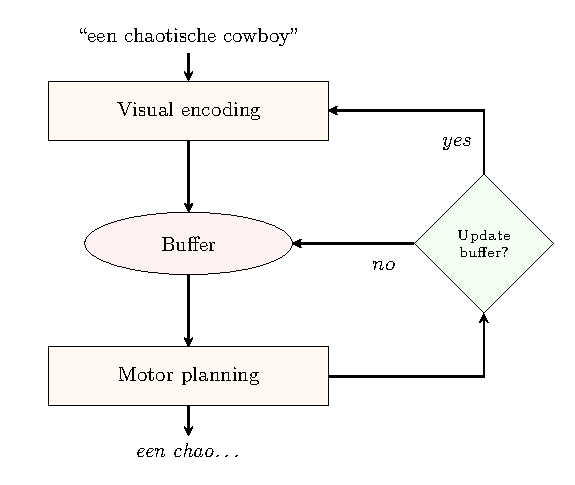
\includegraphics[scale=.7]{spelling_decision.pdf}
	\end{center}
	
\end{frame}

